% Los warning que da son de que no se puede ajustar bien el texto que se encuentra en las cajitas

\documentclass{beamer}
\usepackage[utf8]{inputenc}
\usepackage{xcolor}
\usepackage{tcolorbox}
\usepackage{wrapfig}
\usepackage{lipsum}
\usepackage[spanish]{babel}

\begin{document}

\begin{frame}{Minipage}
\begin{minipage}[l]{0.45\textwidth}

\includegraphics[width=\textwidth]{paisaje}
\end{minipage}
\begin{minipage}[r]{0.5\textwidth}
Una foto Portocolom que muestra {\bf Es Rivetó}, cpm sis características {\em barracas}, como las llamamos, aunque que en otros lugares las llaman {\em escars}, un nombre asociado a un lugar con un plano inclinado para extraer las barcas.
\end{minipage}
\end{frame}


\begin{frame}{Minipage con fbox}
\section{Minipage con fbox}
\fbox{\begin{minipage}[l]{0.5\textwidth}
Una foto Portocolom que muestra {\bf Es Rivetó}, con sus características {\em barracas}, como las llamamos, aunque que en otros lugares las llaman {\em escars}, un nombre asociado a un lugar con un plano inclinado para extraer las barcas.
\end{minipage}}
\begin{minipage}[r]{0.45\textwidth}

\includegraphics[width=\textwidth]{paisaje}
\end{minipage}
\end{frame}


\begin{frame}{Minipage con fbox y colorbox}
\section{Minipage con fbox}
\fbox{\colorbox{green}{\begin{minipage}[l]{0.47\textwidth}
Una foto Portocolom que muestra {\bf Es Rivetó}, con sus características {\em barracas}, como las llamamos, aunque que en otros lugares las llaman {\em escars}, un nombre asociado a un lugar con un plano inclinado para extraer las barcas.
\end{minipage}}}
\begin{minipage}[r]{0.47\textwidth}

\includegraphics[width=\textwidth]{paisaje}
\end{minipage}
\end{frame}


\begin{frame}{Minipage con tcolorbox}
\begin{tcolorbox}
\begin{minipage}[l]{0.45\textwidth}
Una foto Portocolom que muestra {\bf Es Rivetó}, con sus características {\em barracas}, como las llamamos, aunque que en otros lugares las llaman {\em escars}, un nombre asociado a un lugar con un plano inclinado para extraer las barcas.
\end{minipage}
\begin{minipage}[r]{0.45\textwidth}

\includegraphics[width=\textwidth]{paisaje}
\end{minipage}
\end{tcolorbox}
\end{frame}


\begin{frame}{Wrapfigure (requiere el paquete wrapfig)}
\begin{wrapfigure}[10]{l}{0.4\textwidth}
\begin{center}
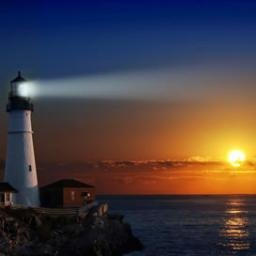
\includegraphics[width=0.4\textwidth]{faro.jpg}
\end{center}
%\caption{Es Faro} % sale por superpuesto con el texto
\end{wrapfigure}
\noindent
{\small \lipsum[0-1]}
\end{frame}


\begin{frame}{Un reto}
¿Como sería el código en \LaTeX para una composición con tres recuadros como estos:
\newline
\fbox{\colorbox{magenta}{\begin{minipage}[l]{3cm}Una foto de Portocolom que muestra {\bf Es Rivetó}, con sus características {\em barracas} o {\em escars}, un nombre asociado a un lugar con un plano inclinado para extraer las barcas.
\end{minipage}}}
\fbox{\begin{minipage}[c]{3cm}Una foto de Portocolom que muestra {\bf Es Rivetó}, con sus características {\em barracas} o {\em escars}, un nombre asociado a un lugar con un plano inclinado para extraer las barcas.
\end{minipage}}
\fbox{\colorbox{cyan}{\begin{minipage}[r]{3cm}Una foto de Portocolom que muestra {\bf Es Rivetó}, con sus características {\em barracas} o {\em escars}, un nombre asociado a un lugar con un plano inclinado para extraer las barcas.
\end{minipage}}}
\end{frame}

\end{document}